\section{Results}\label{sec:results}

\subsection{Common-window ranking}\label{subsec:ranking-results}

All experiments were evaluated on the same validation window defined in
Section~\ref{subsec:data-protocol}. Table~\ref{tab:ranking} and
Fig.~\ref{fig:metric-ranking} show a clear separation between the
physical-only baselines, the pure ML baseline and the hybrid
configurations. The deterministic and stochastic physical baselines
(E0--E3) clustered within a narrow NSE range of 0.414--0.438, whereas
the pure forcing-based ML model (E4) reached NSE\,=\,0.575. All hybrid
models exceeded E4 in NSE, indicating that the stochastic physical
ensemble supplied additional predictive information beyond the observed
forcing variables alone.

The strongest \emph{backend-consistent} configuration was
E6\_HYB\_XGB\_QUANTILES, which achieved NSE\,=\,0.740,
KGE\,=\,0.810, RMSE\,=\,0.275~m$^3$\,s$^{-1}$,
MAE\,=\,0.162~m$^3$\,s$^{-1}$ and PBIAS\,=\,0.927\%. This run is the
main evidence for the proposed quantile-based stochastic physical--ML
hybridization because its manuscript label and executed backend are
consistent. The numerically best run was E8\_HYB\_GRU\_QUANTILES
(NSE\,=\,0.849, KGE\,=\,0.899 and RMSE\,=\,0.210~m$^3$\,s$^{-1}$),
but it is interpreted separately because the audit showed that it ran
as a fallback multilayer perceptron on flattened sequences rather than
as a recurrent GRU. The ranking is therefore reported in two layers:
E8 is the best numerical configuration, whereas E6 is the strongest
robust configuration for defensible process-based interpretation.

\begin{table*}[t]
\caption{Final common-window ranking. Metrics are computed on 4367
validation samples from 8 January 2009 to 31 December 2020.}
\label{tab:ranking}
\centering
\small
\begin{tabular*}{\textwidth}{@{\extracolsep{\fill}}rlllllll@{}}
\toprule
Rank & Experiment & NSE & KGE & RMSE & MAE & PBIAS & Backend \\
\midrule
1 & E8\_HYB\_GRU\_QUANTILES   & 0.849 & 0.899 & 0.210 & 0.124
  & 1.579 & fallback\_mlp\_on\_flattened\_sequences \\
2 & E6\_HYB\_XGB\_QUANTILES   & 0.740 & 0.810 & 0.275 & 0.162
  & 0.927 & sklearn\_hgb \\
3 & E7\_HYB\_GRU\_MEAN        & 0.686 & 0.789 & 0.302 & 0.192
  & 1.644 & fallback\_mlp\_on\_flattened\_sequences \\
4 & E5\_HYB\_XGB\_MEAN        & 0.626 & 0.715 & 0.330 & 0.210
  & 2.007 & sklearn\_hgb \\
5 & E4\_ML\_PURE\_XGB         & 0.575 & 0.661 & 0.352 & 0.223
  & 0.742 & sklearn\_hgb \\
6 & E1\_RAMIS\_DET\_BF        & 0.438 & 0.714 & 0.405 & 0.248
  & 0.860 & physical \\
7 & E3\_RAMIS\_LEVY\_BF       & 0.429 & 0.725 & 0.408 & 0.255
  & -1.218 & physical \\
8 & E2\_RAMIS\_LEVY\_NOBF     & 0.427 & 0.717 & 0.409 & 0.268
  & -7.551 & physical \\
9 & E0\_RAMIS\_DET\_NOBF      & 0.414 & 0.713 & 0.413 & 0.270
  & -5.865 & physical \\
\bottomrule
\end{tabular*}
\end{table*}

\begin{figure}[t]
\centering
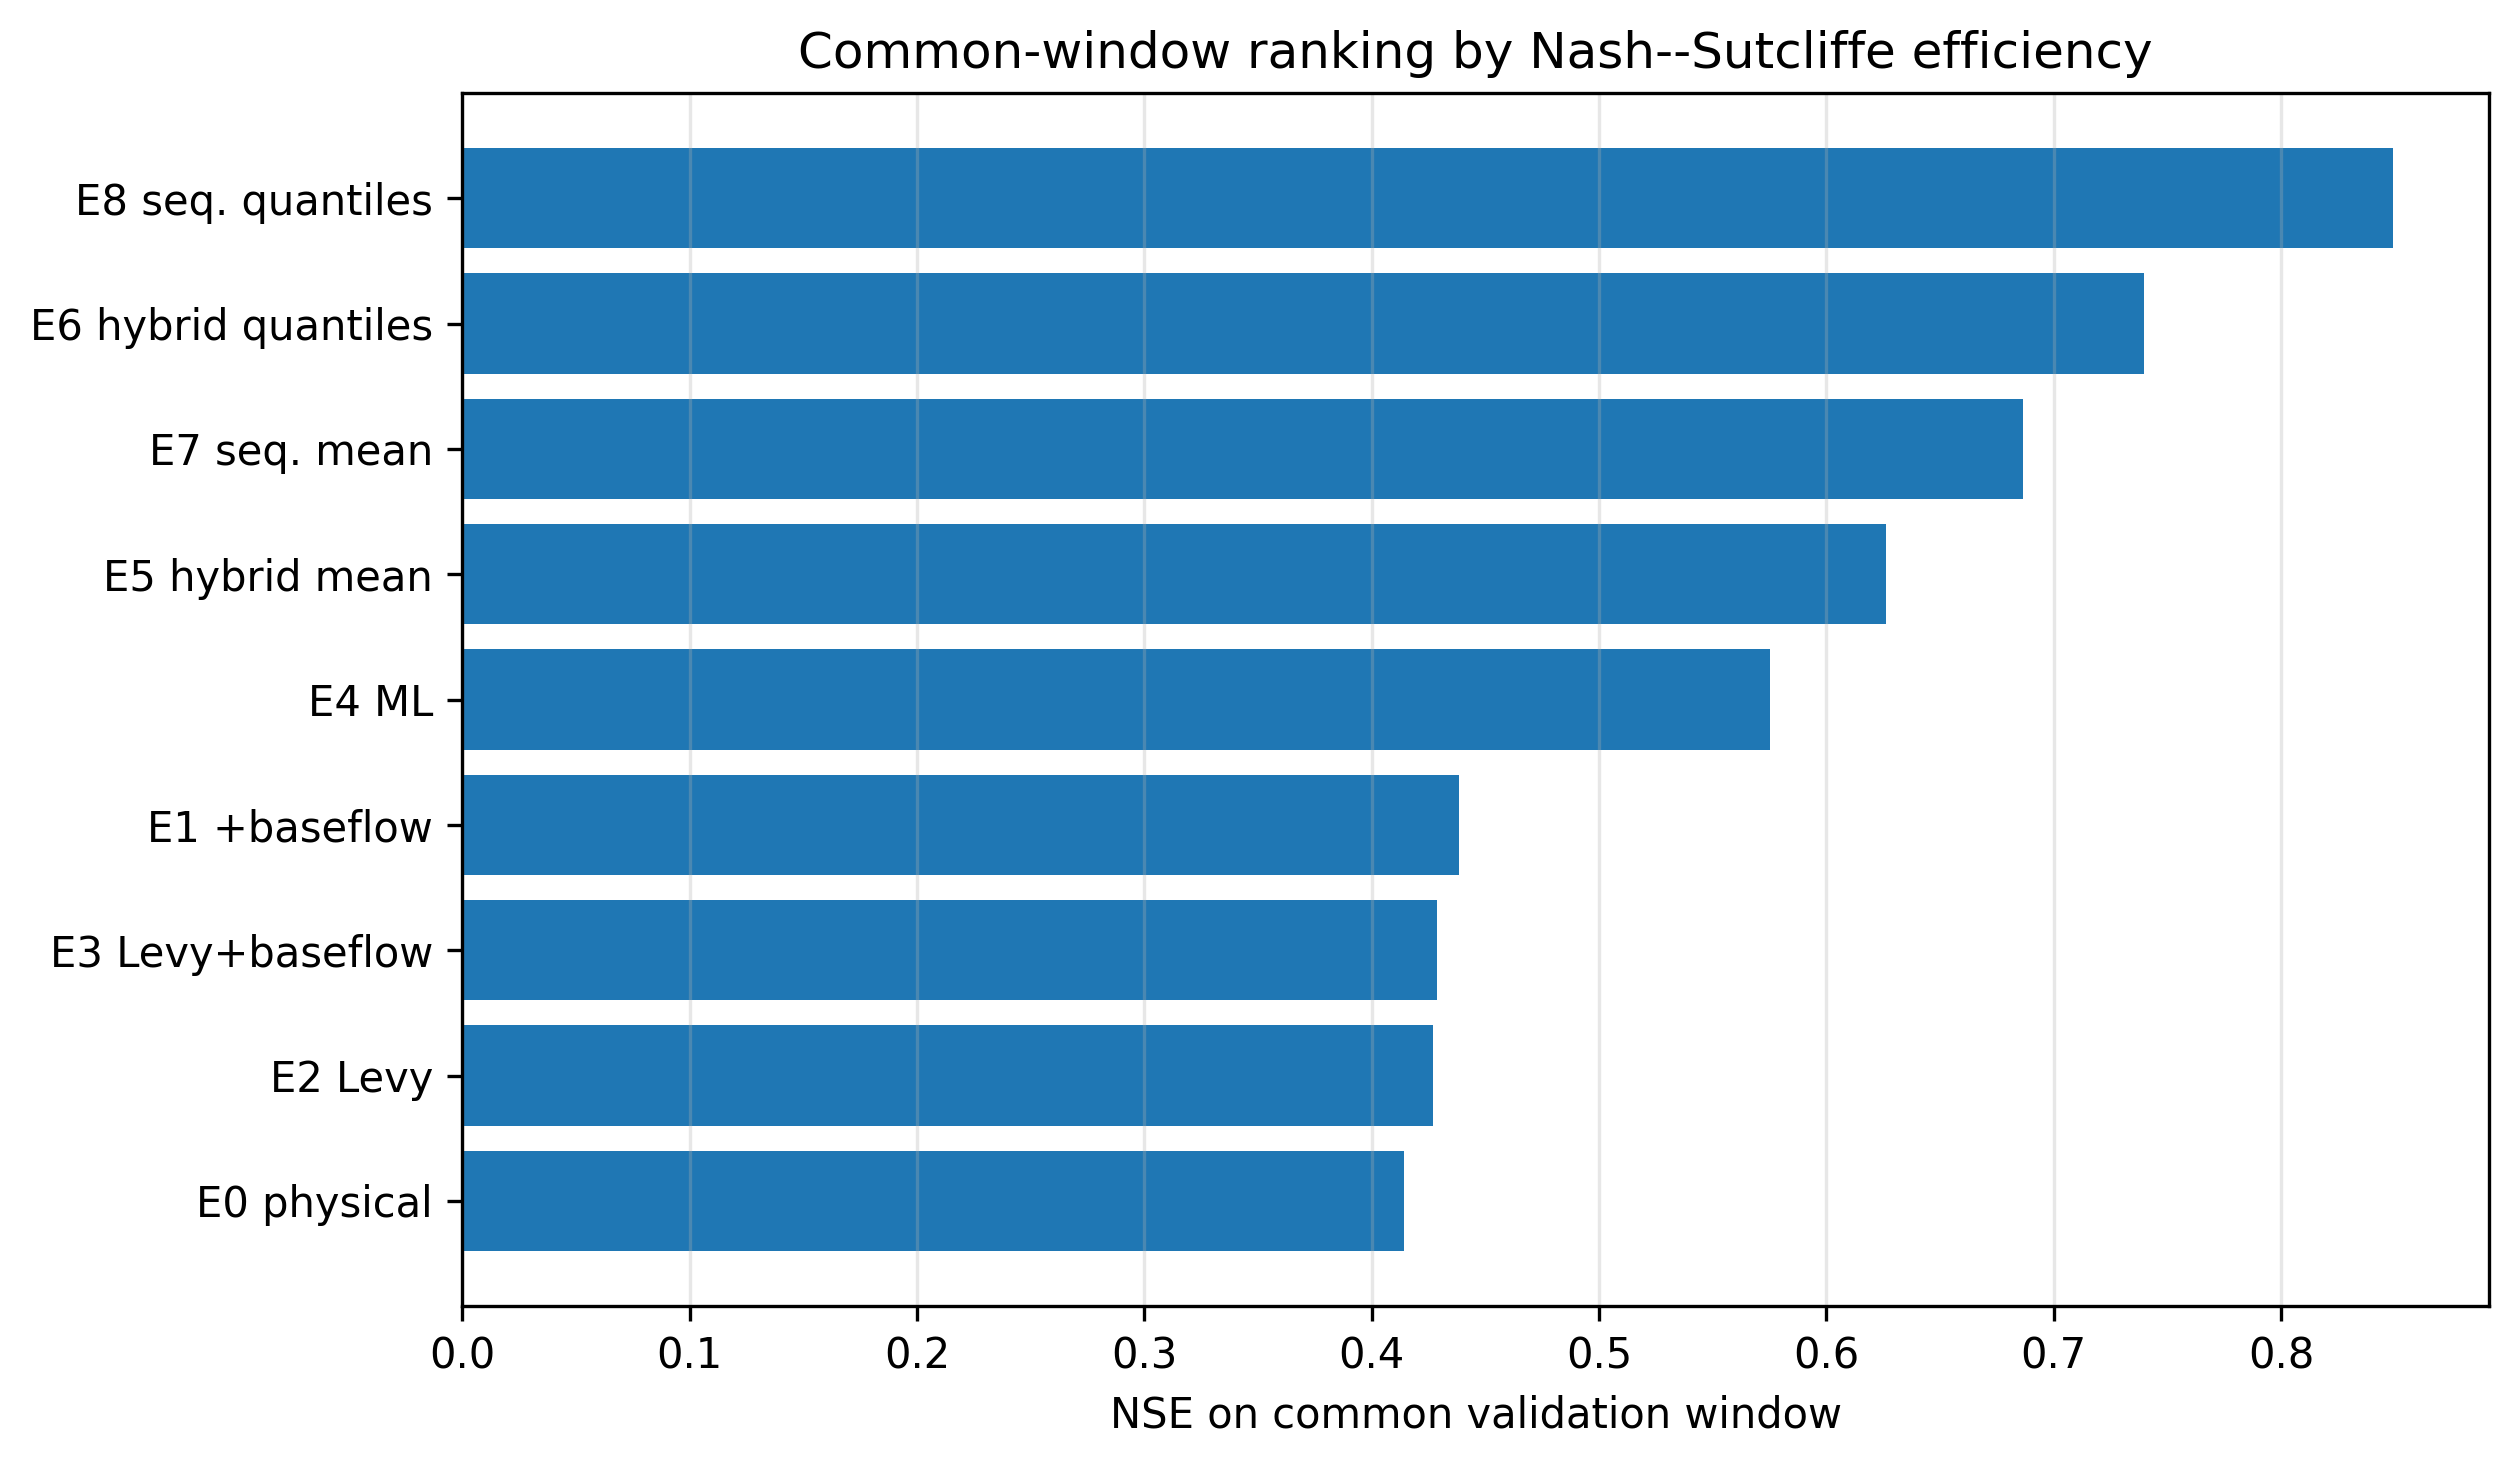
\includegraphics[width=0.95\linewidth]{figures/metric_ranking_nse.png}
\caption{Ranking of all experiments by common-window NSE. Numerical
values correspond to Table~\ref{tab:ranking}.}
\label{fig:metric-ranking}
\end{figure}

\subsection{Hydrograph and flow-duration behaviour}
\label{subsec:hydro-results}

The validation hydrograph in Fig.~\ref{fig:hydrograph-common} shows
that the hybrid models reproduce the timing and amplitude of seasonal
streamflow fluctuations more closely than the physical-only baselines.
The physical models retain the main wet-season response but frequently
collapse towards near-zero discharge during recession periods. This
behaviour is also evident in the flow-duration curves
(Fig.~\ref{fig:fdc-common}), where E0 shows an unrealistic decline in
the high-exceedance tail. Adding the baseflow reservoir reduces this
problem only partially, indicating that the single linear storage term
improves recession persistence but does not fully resolve dry-season
memory.

The hybrid configurations provide a closer match to the observed
flow-duration curve over most exceedance probabilities. The largest
visual improvement occurs in the lower-flow tail, where quantile-based
hybrids avoid the extreme collapse of the deterministic physical
trajectory. Nevertheless, the hydrograph also shows remaining errors
during sharp wet-season peaks. Thus, the hybrid improvement is not a
complete correction of event-scale dynamics; it is mainly a reduction
of systematic distributional errors and dry-season underestimation.

\begin{figure*}[t]
\centering
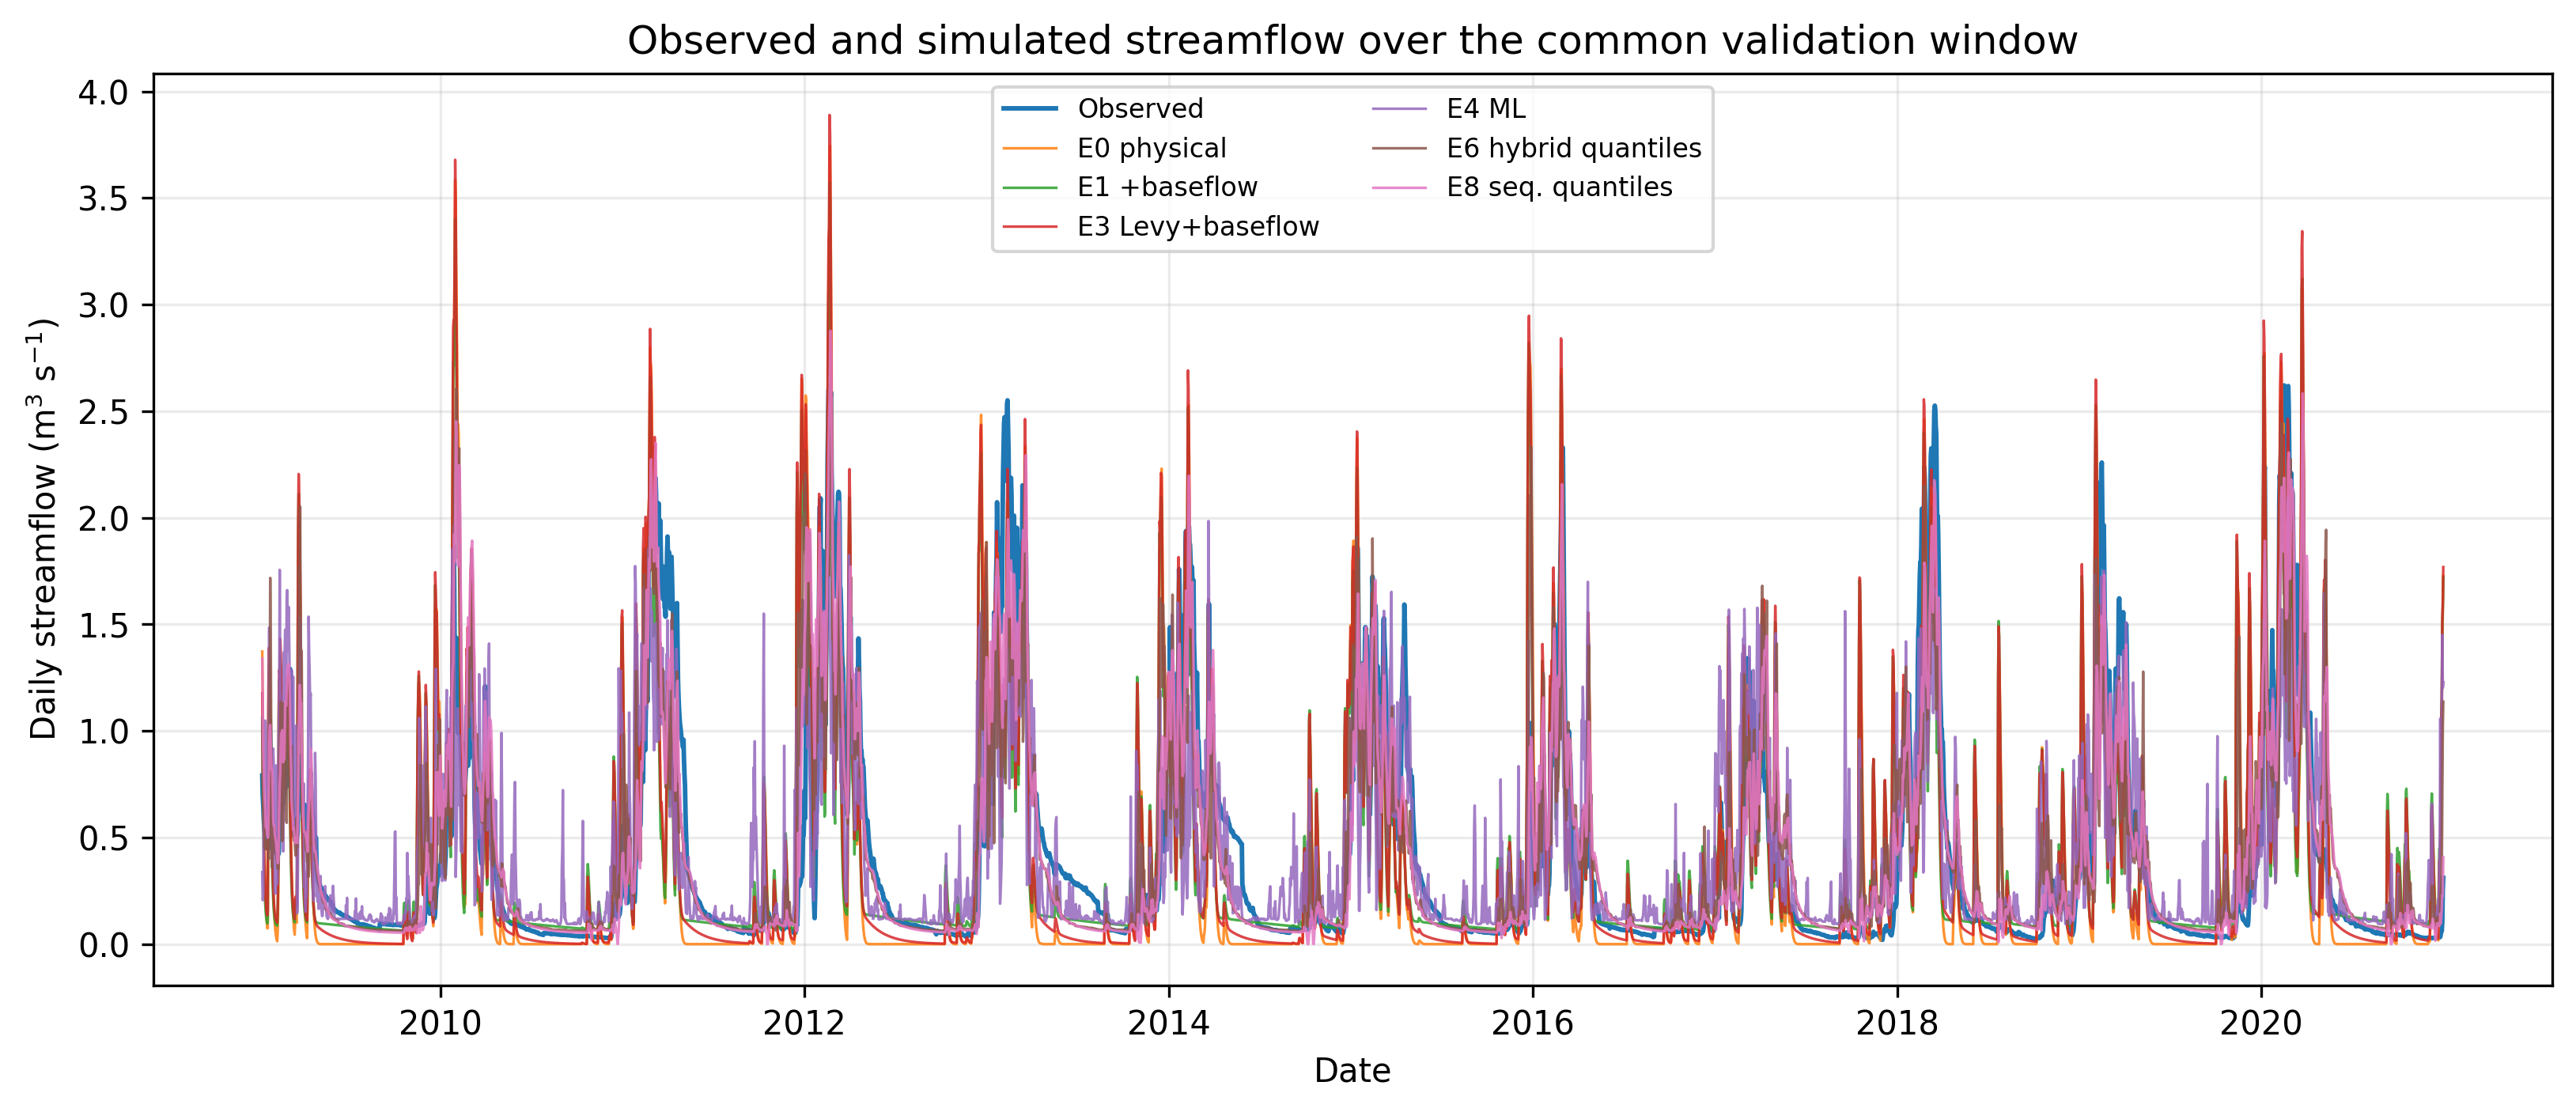
\includegraphics[width=0.98\textwidth]{figures/hydrograph_validation_common.png}
\caption{Observed and simulated daily discharge over the common
validation window for representative physical, pure ML and hybrid
models.}
\label{fig:hydrograph-common}
\end{figure*}

\begin{figure}[t]
\centering
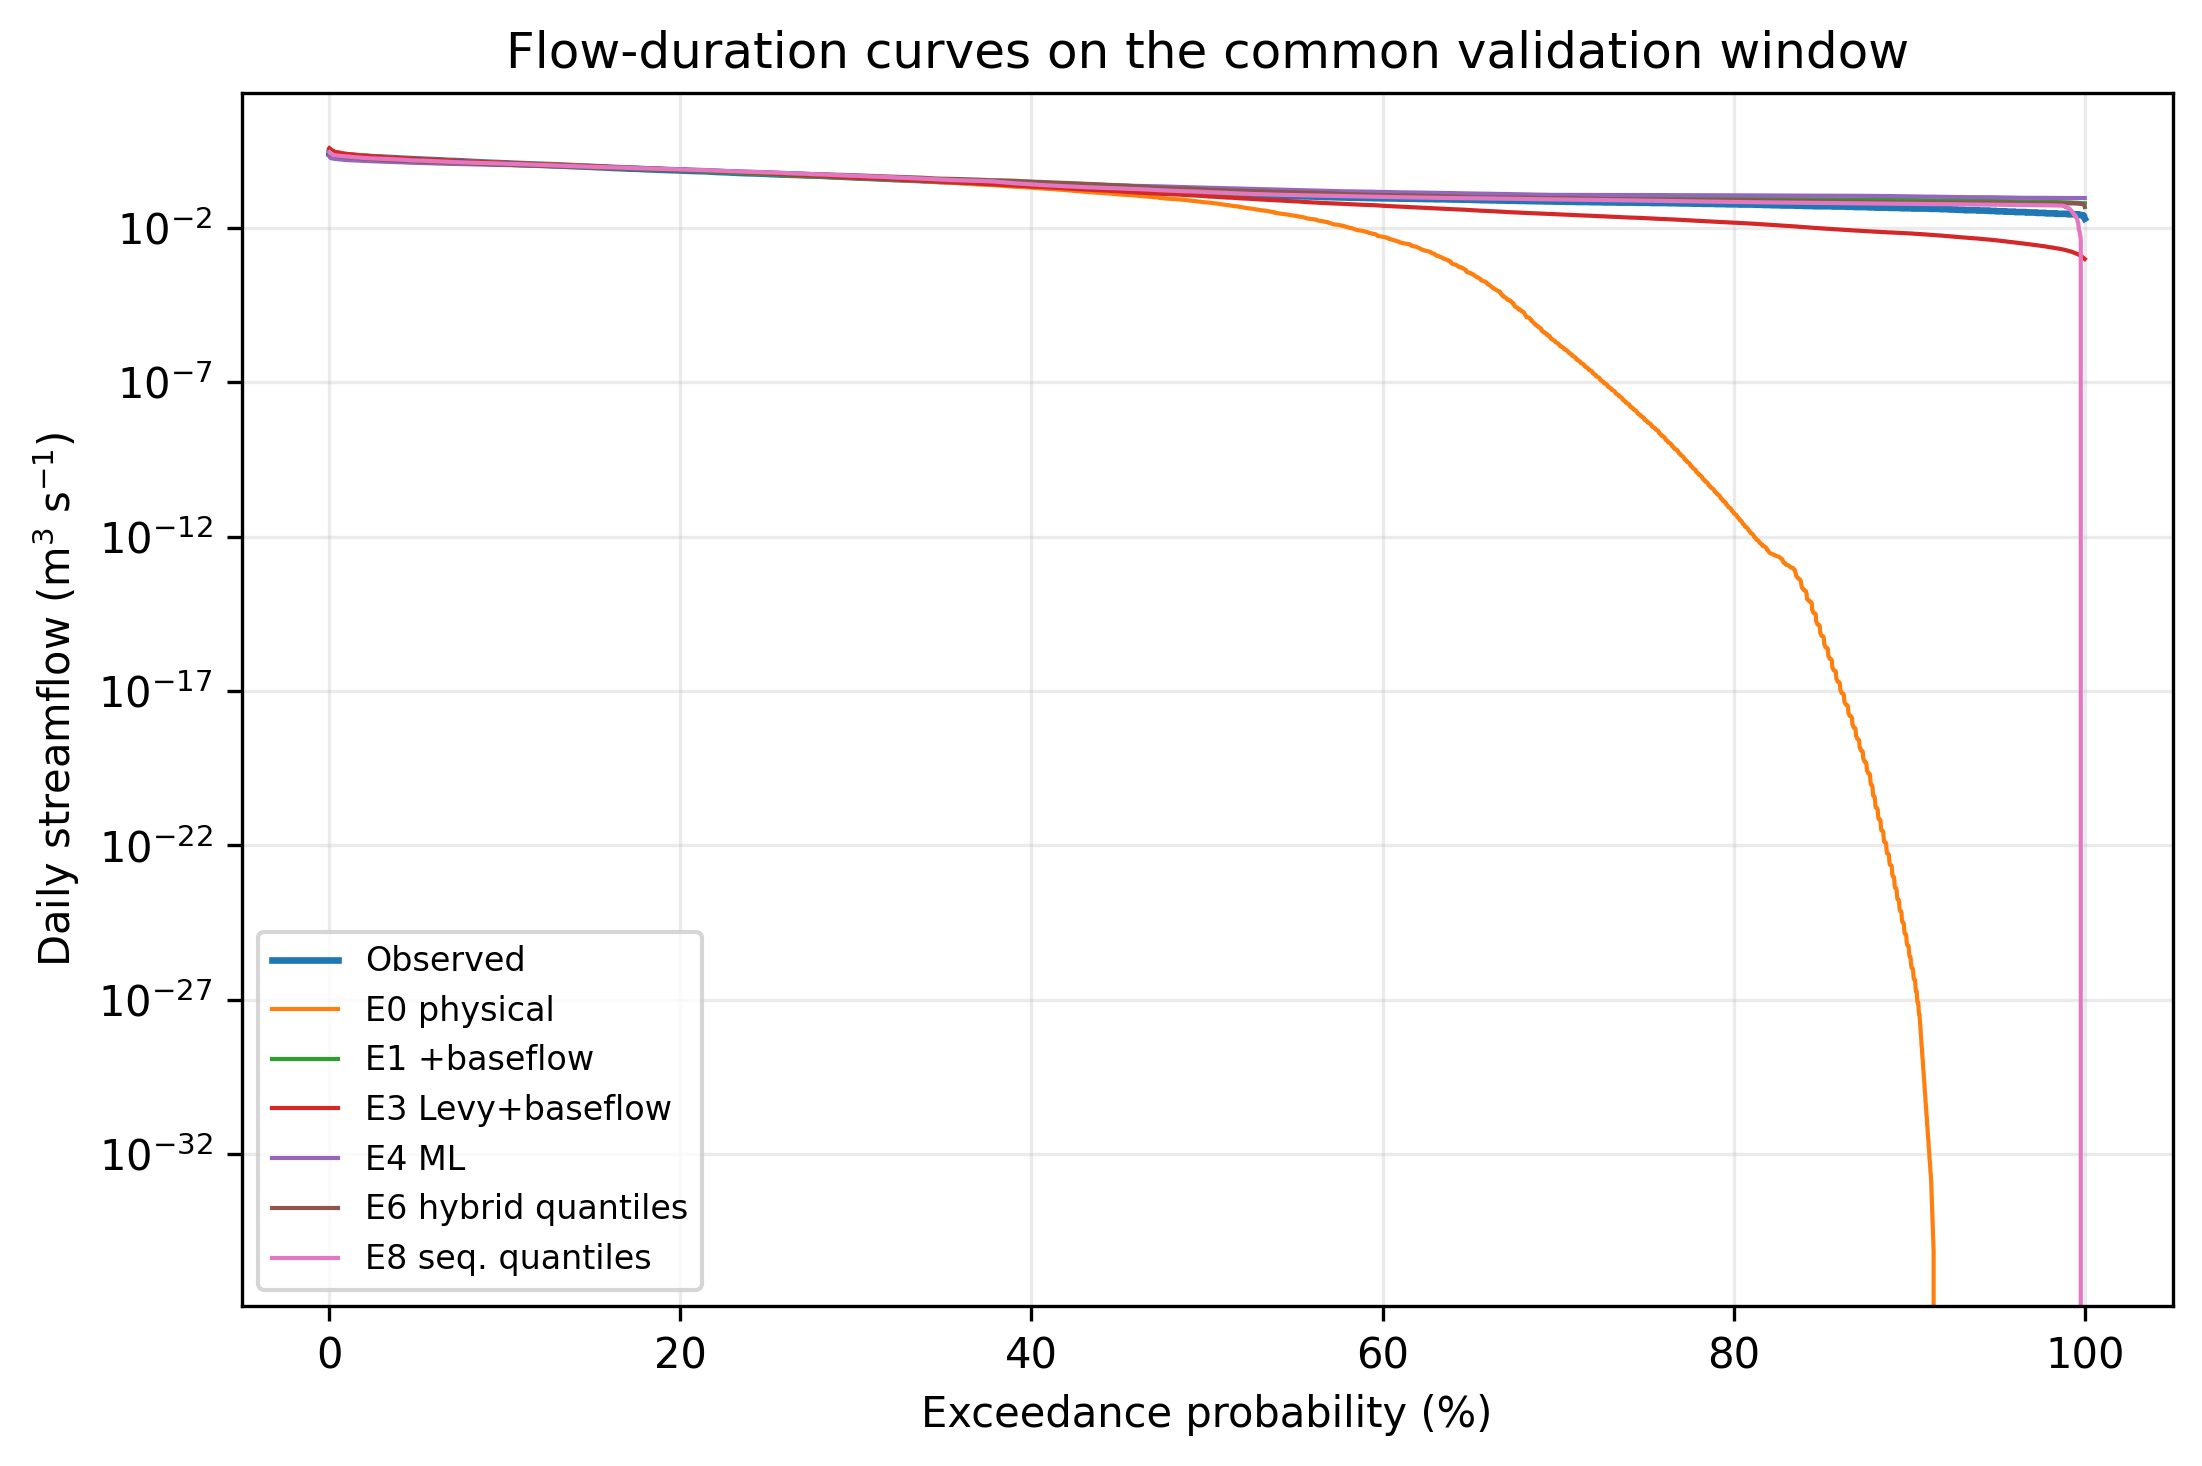
\includegraphics[width=0.95\linewidth]{figures/fdc_common.png}
\caption{Flow-duration curves for observed discharge and representative
simulations over the common validation window.}
\label{fig:fdc-common}
\end{figure}

\subsection{Ablation effects}\label{subsec:ablation-results}

Table~\ref{tab:ablation} and Fig.~\ref{fig:ablation-effects} isolate
the contribution of each modelling component. Adding the baseflow
reservoir to the deterministic physical model increased NSE by 0.024
and reduced RMSE by 0.009~m$^3$\,s$^{-1}$ (E1--E0). Under stochastic
forcing, the same structural addition produced a smaller but still
positive gain in NSE and KGE (E3--E2). In contrast, adding
L\'{e}vy-type perturbations to the baseflow-enabled physical model did
not improve point-prediction skill: NSE decreased by 0.010 and RMSE
increased by 0.004~m$^3$\,s$^{-1}$, although KGE increased slightly.
This confirms that stochastic perturbation is not, by itself, the main
source of point-prediction improvement.

The dominant gain came from hybridization. Relative to the complete
stochastic physical baseline (E3), the pure forcing-based ML model
(E4) improved NSE by 0.147, whereas the XGB-labelled hybrid using
ensemble means (E5) improved NSE by 0.198. The quantile-based hybrid
(E6) produced the largest backend-consistent ablation effect, with
$\Delta$NSE\,=\,0.311 and $\Delta$RMSE\,=\,-0.133~m$^3$\,s$^{-1}$
relative to E3. The direct comparison between E6 and E5 added
0.114 NSE and 0.095 KGE, showing that ensemble quantiles carry useful
predictive information that is lost when the stochastic physical
ensemble is compressed to its mean alone.

The GRU-labelled contrasts must be interpreted with the backend audit
in mind. E7 and E8 improved over their XGB-labelled counterparts, but
these gains cannot be attributed to recurrent-network memory because
both runs used a fallback MLP backend. They are therefore reported as
additional sequential-feature experiments under fallback execution, not
as evidence that GRU architecture is superior.

\begin{table*}[t]
\caption{Ablation effects on the common validation window. Positive
$\Delta$NSE and $\Delta$KGE indicate improvement; negative
$\Delta$RMSE and $\Delta$MAE indicate error reduction.}
\label{tab:ablation}
\centering
\small
\begin{tabular*}{\textwidth}{@{\extracolsep{\fill}}lllrrrr@{}}
\toprule
Ablation & Baseline & Candidate
  & $\Delta$NSE & $\Delta$KGE & $\Delta$RMSE & $\Delta$MAE \\
\midrule
deterministic\_baseflow
  & E0\_RAMIS\_DET\_NOBF & E1\_RAMIS\_DET\_BF
  & 0.024 & 0.000 & -0.009 & -0.022 \\
stochastic\_baseflow
  & E2\_RAMIS\_LEVY\_NOBF & E3\_RAMIS\_LEVY\_BF
  & 0.002 & 0.008 & -0.001 & -0.012 \\
levy\_given\_baseflow
  & E1\_RAMIS\_DET\_BF & E3\_RAMIS\_LEVY\_BF
  & -0.010 & 0.011 & 0.004 & 0.008 \\
pure\_ml\_vs\_physical
  & E3\_RAMIS\_LEVY\_BF & E4\_ML\_PURE\_XGB
  & 0.147 & -0.064 & -0.056 & -0.033 \\
hybrid\_mean\_vs\_physical
  & E3\_RAMIS\_LEVY\_BF & E5\_HYB\_XGB\_MEAN
  & 0.198 & -0.010 & -0.078 & -0.046 \\
hybrid\_quantiles\_vs\_physical
  & E3\_RAMIS\_LEVY\_BF & E6\_HYB\_XGB\_QUANTILES
  & 0.311 & 0.085 & -0.133 & -0.094 \\
quantiles\_vs\_mean\_xgb
  & E5\_HYB\_XGB\_MEAN & E6\_HYB\_XGB\_QUANTILES
  & 0.114 & 0.095 & -0.055 & -0.048 \\
gru\_mean\_vs\_xgb\_mean
  & E5\_HYB\_XGB\_MEAN & E7\_HYB\_GRU\_MEAN
  & 0.060 & 0.074 & -0.028 & -0.018 \\
gru\_quantiles\_vs\_xgb\_quantiles
  & E6\_HYB\_XGB\_QUANTILES & E8\_HYB\_GRU\_QUANTILES
  & 0.109 & 0.089 & -0.066 & -0.038 \\
\bottomrule
\end{tabular*}
\end{table*}

\begin{figure}[t]
\centering
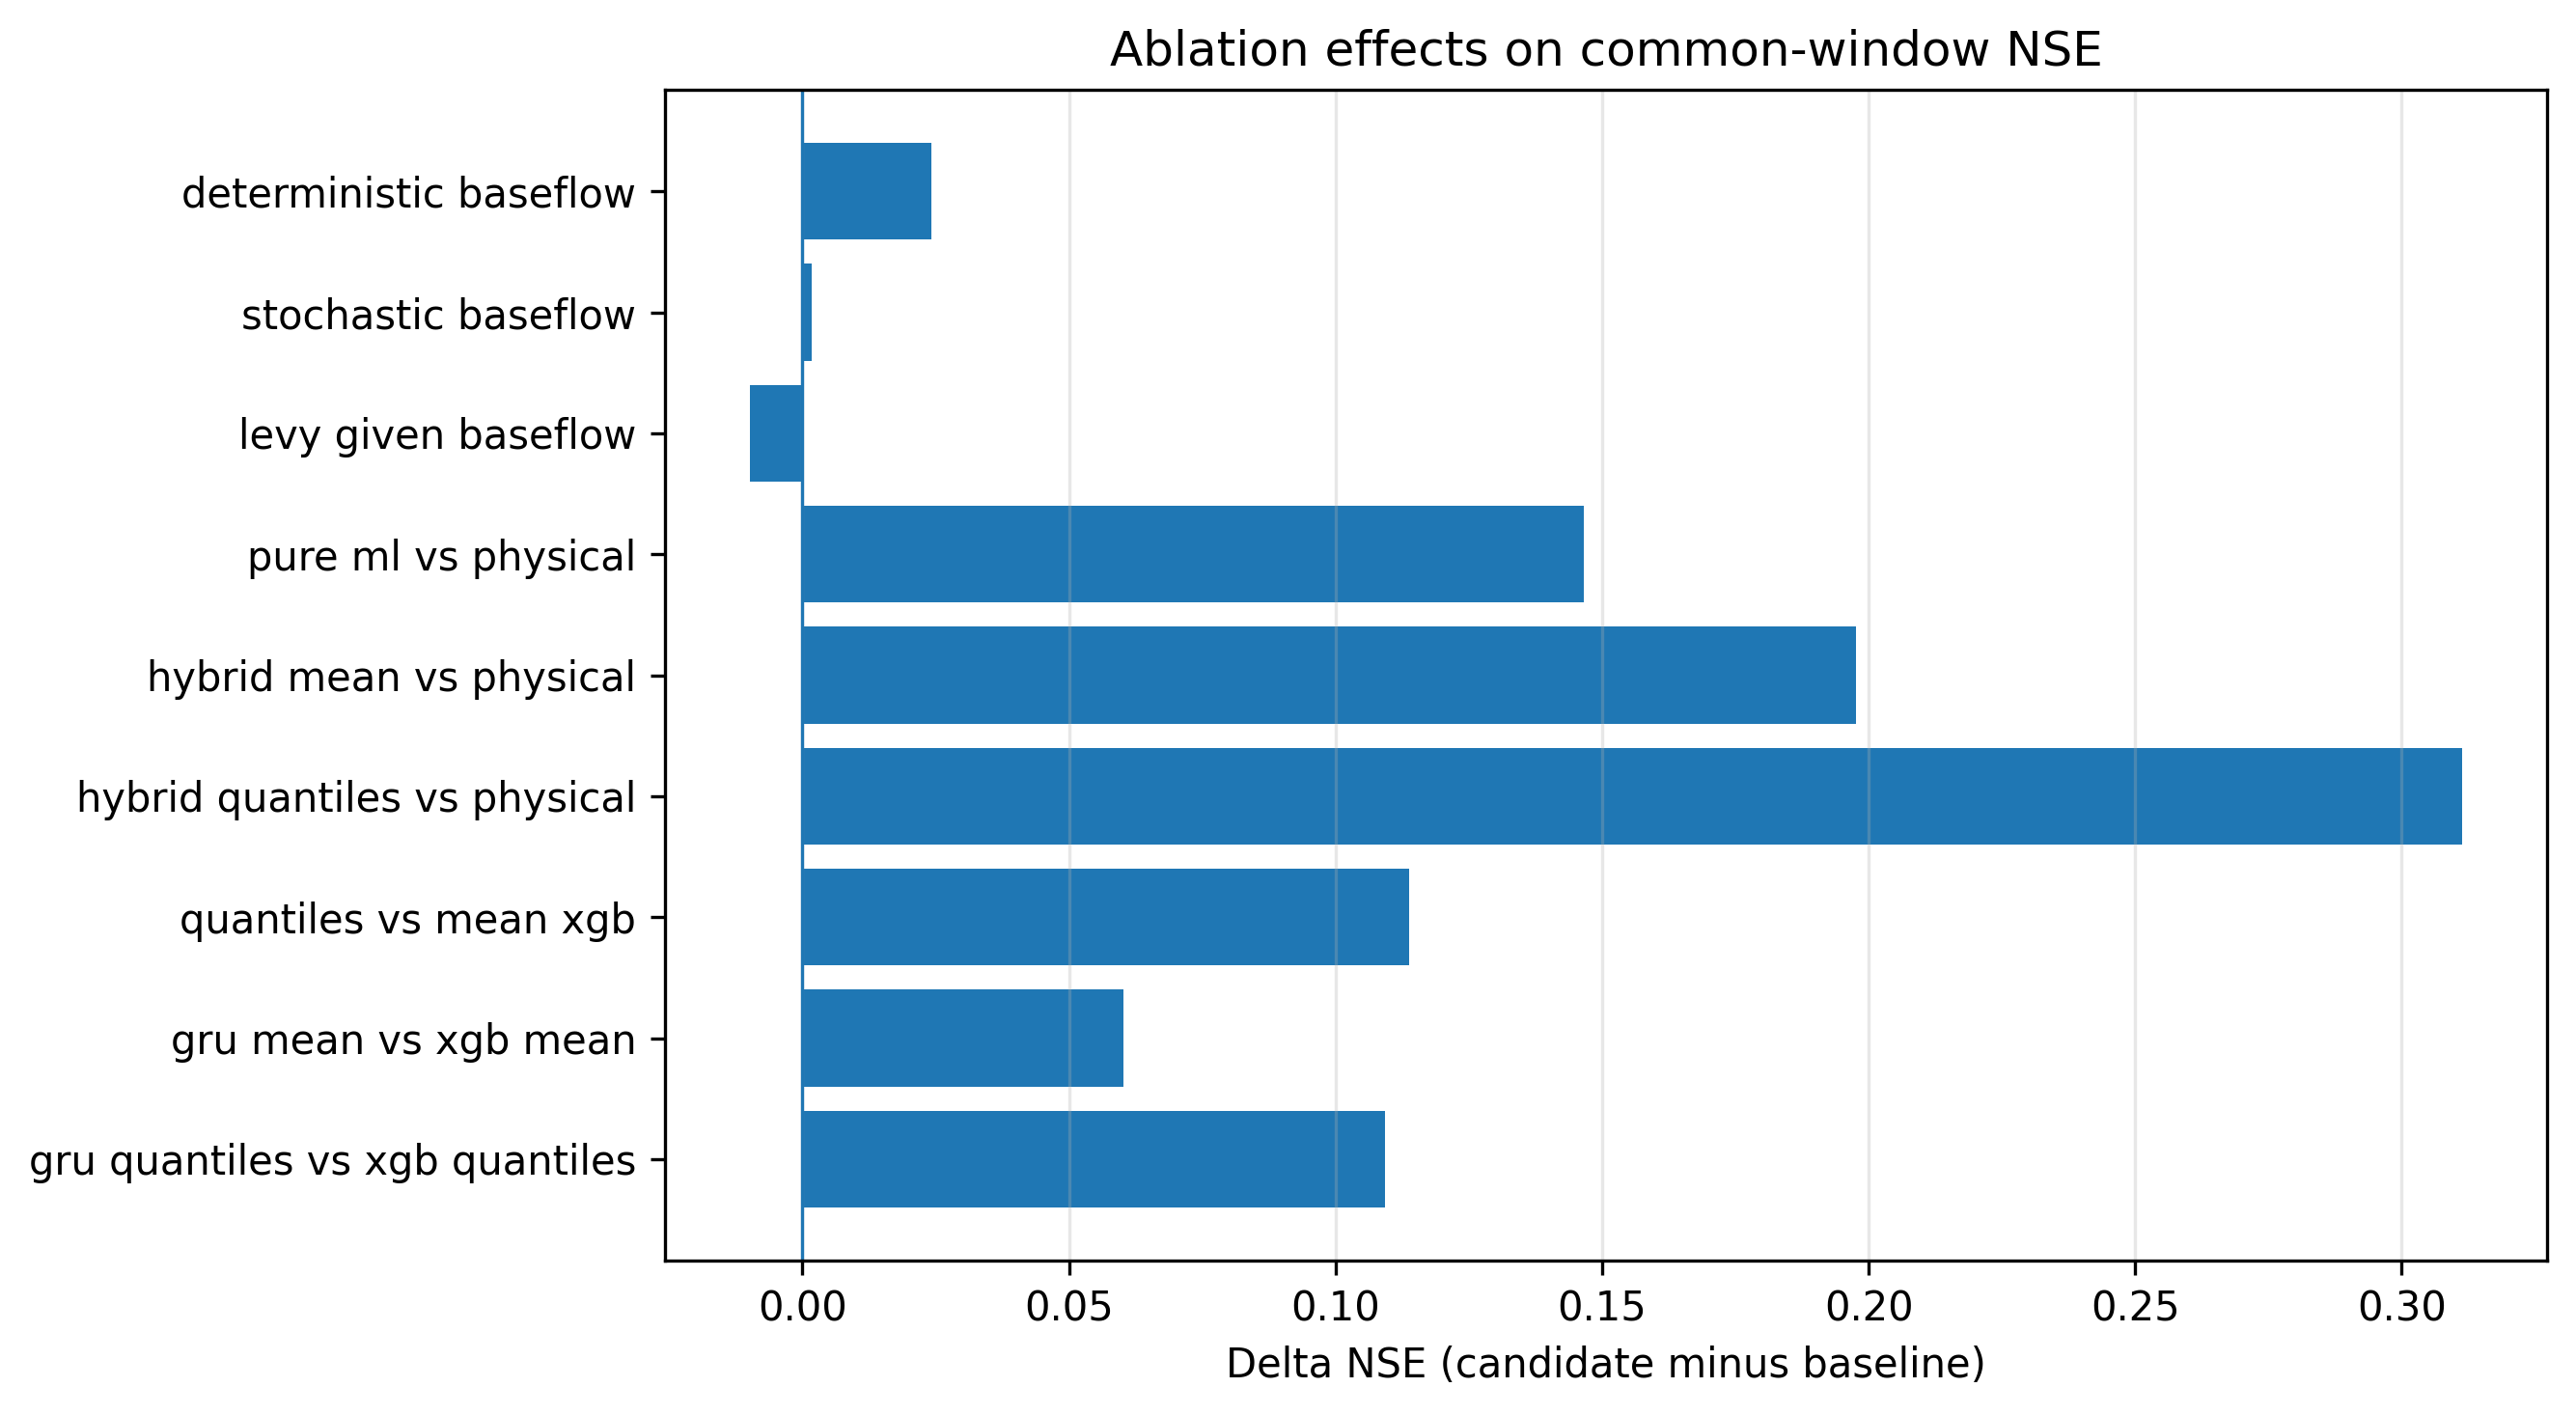
\includegraphics[width=0.95\linewidth]{figures/ablation_effects.png}
\caption{Ablation effects expressed as candidate-minus-baseline
$\Delta$NSE. Numerical values are reported in Table~\ref{tab:ablation}.}
\label{fig:ablation-effects}
\end{figure}

\subsection{Performance by flow regime}\label{subsec:regime-results}

Regime-specific RMSE values (Table~\ref{tab:regime-rmse} and
Fig.~\ref{fig:regime-rmse}) show that model skill is strongly
flow-dependent. The physical-only configurations had similar errors
across the selected regimes, with the largest absolute errors in the
high-flow class. The pure ML model reduced mid-flow RMSE relative to
the physical baselines, but its low-flow RMSE remained close to that of
the physical models. The quantile-based hybrid E6 substantially reduced
errors in all regimes, and the numerically best E8 configuration
further reduced RMSE under fallback-MLP execution.

The largest proportional improvement occurred in the low-flow regime:
RMSE decreased from 0.177~m$^3$\,s$^{-1}$ for E0 to
0.075~m$^3$\,s$^{-1}$ for E6 and 0.047~m$^3$\,s$^{-1}$ for E8. The
mid-flow and high-flow regimes also improved, but larger residual
errors persisted during high flows, where event timing and peak
magnitude remain more difficult to reproduce. These results support the
interpretation from the flow-duration curves: stochastic ensemble
quantiles are most useful for correcting systematic distributional
errors, especially during recession and low-flow periods, while peak
simulation remains only partially corrected.

\begin{table}[t]
\caption{RMSE (m$^3$\,s$^{-1}$) by flow regime for representative
models. Regime thresholds were estimated from calibration observations
only.}
\label{tab:regime-rmse}
\centering
\small
\begin{tabular*}{\linewidth}{@{\extracolsep{\fill}}lrrr@{}}
\toprule
Experiment & Low & Mid & High \\
\midrule
E0\_RAMIS\_DET\_NOBF   & 0.177 & 0.392 & 0.615 \\
E1\_RAMIS\_DET\_BF     & 0.197 & 0.365 & 0.613 \\
E3\_RAMIS\_LEVY\_BF    & 0.185 & 0.387 & 0.604 \\
E4\_ML\_PURE\_XGB      & 0.189 & 0.276 & 0.566 \\
E6\_HYB\_XGB\_QUANTILES & 0.075 & 0.222 & 0.461 \\
E8\_HYB\_GRU\_QUANTILES & 0.047 & 0.171 & 0.352 \\
\bottomrule
\end{tabular*}
\end{table}

\begin{figure}[t]
\centering
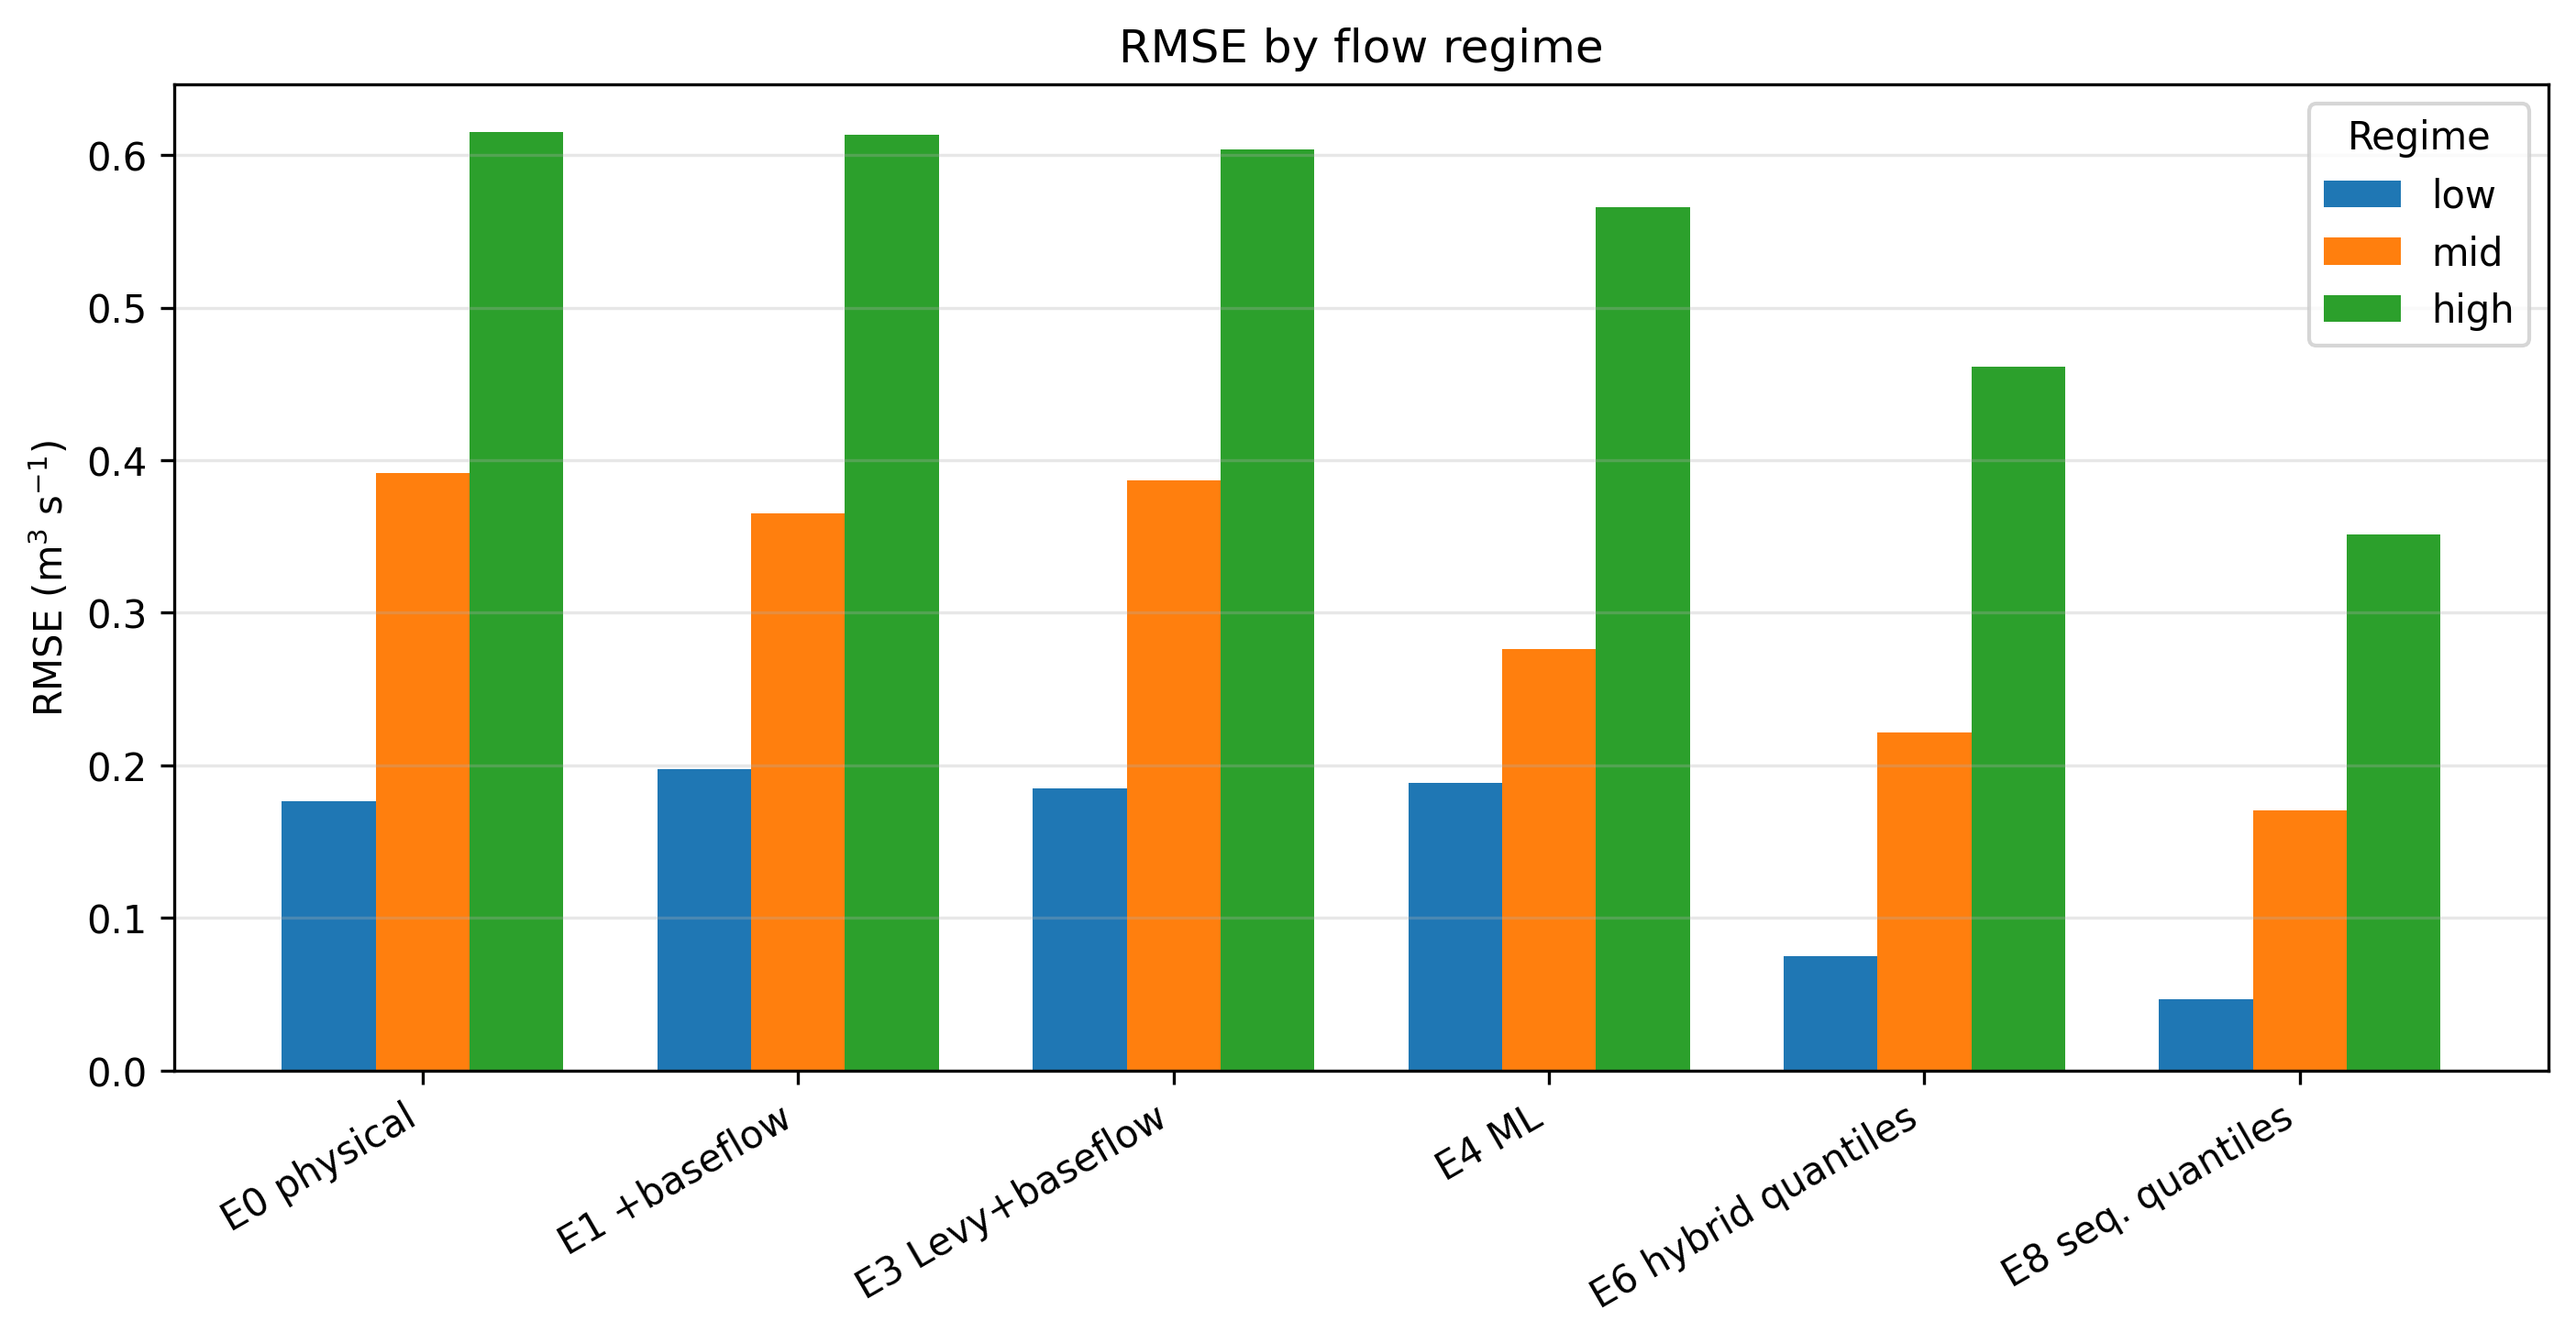
\includegraphics[width=0.95\linewidth]{figures/regime_rmse.png}
\caption{RMSE by low, mid and high flow regimes for representative
models. Values correspond to Table~\ref{tab:regime-rmse}.}
\label{fig:regime-rmse}
\end{figure}

\subsection{Uncertainty diagnostics and backend audit}
\label{subsec:uncertainty-results}

The stochastic physical intervals were strongly underdispersive
(Table~\ref{tab:uncertainty} and Fig.~\ref{fig:uncertainty-diagnostics}).
E2 achieved PICP\,=\,0.160 and E3 achieved PICP\,=\,0.004, both far
below the nominal 0.95 target. The corresponding PINAW values were also
small, particularly for E3 (PINAW\,=\,0.003), indicating that the
intervals were narrow rather than reliably calibrated. The high Winkler
scores confirm that most observed values fell outside the nominal
intervals. Consequently, the stochastic ensemble should not be reported
as a calibrated predictive uncertainty product in its current form. Its
main demonstrated value is as a source of physically structured
features for ML correction.

Table~\ref{tab:backend} summarizes the backend audit. The XGB-labelled
experiments (E4--E6) used the \texttt{sklearn\_hgb} backend, whereas
the GRU-labelled experiments (E7 and E8) used
\texttt{fallback\_mlp\_on\_flattened\_sequences}. This distinction
changes the interpretation of the leaderboard: E8 may be reported as
the best numerical experiment, but not as evidence for recurrent neural
networks. The reproducibility checklist in
Table~\ref{tab:reproducibility} returned no FAIL item. WARN items were
associated with missing observed-flow values, low-flow physical
limitations, optional figure entries and the fallback backend, rather
than with direct evidence of temporal leakage.

\begin{table}[t]
\caption{Uncertainty diagnostics for stochastic physical reference
bands.}
\label{tab:uncertainty}
\centering
\small
\begin{tabular*}{\linewidth}{@{\extracolsep{\fill}}lrrrr@{}}
\toprule
Experiment & PICP & PINAW & MPIW & Winkler \\
\midrule
E2\_RAMIS\_LEVY\_NOBF & 0.160 & 0.084 & 0.219 & 7.297 \\
E3\_RAMIS\_LEVY\_BF   & 0.004 & 0.003 & 0.009 & 10.050 \\
\bottomrule
\end{tabular*}
\end{table}

\begin{figure}[t]
\centering
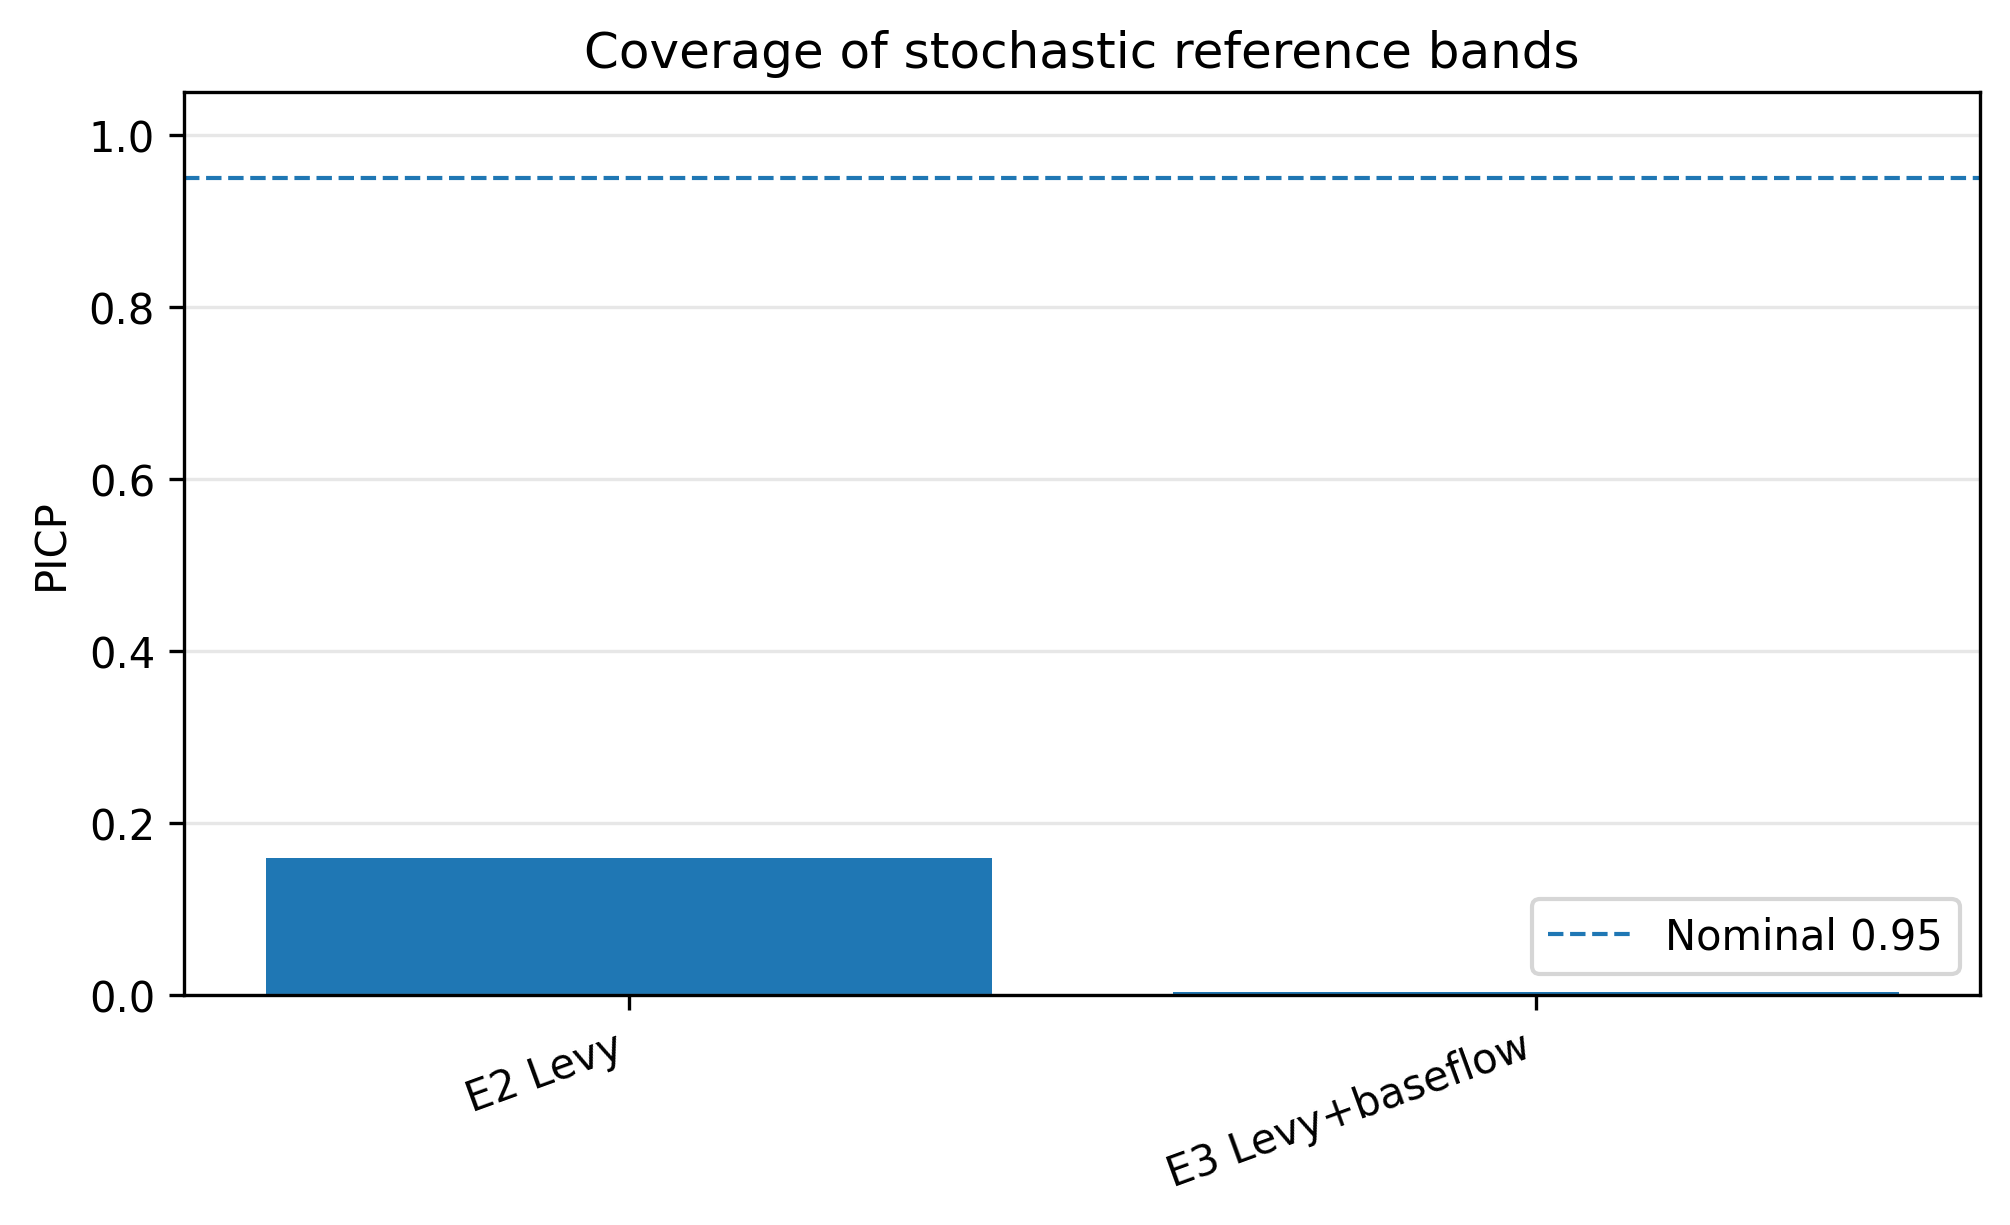
\includegraphics[width=0.95\linewidth]{figures/uncertainty_diagnostics.png}
\caption{Prediction interval coverage probability for stochastic
physical references. The dashed line marks the nominal 0.95 target.}
\label{fig:uncertainty-diagnostics}
\end{figure}

\begin{table*}[t]
\caption{Backend-aware manuscript notes for ML and hybrid configurations.}
\label{tab:backend}
\centering
\small
\begin{tabular*}{\textwidth}{@{\extracolsep{\fill}}p{0.22\textwidth}p{0.10\textwidth}p{0.24\textwidth}p{0.17\textwidth}p{0.20\textwidth}@{}}
\toprule
Experiment & ML label & Backend label & Feature source
  & Manuscript claim \\
\midrule
E4\_ML\_PURE\_XGB      & xgboost & sklearn\_hgb & observed\_forcing
  & report as gradient boosting (HGB) \\
E6\_HYB\_XGB\_QUANTILES & xgboost & sklearn\_hgb & stochastic\_ensemble
  & report as gradient boosting (HGB) \\
E7\_HYB\_GRU\_MEAN     & gru & fallback\_mlp\_on\_flattened\_sequences
  & stochastic\_ensemble & fallback MLP, not real recurrent GRU \\
E8\_HYB\_GRU\_QUANTILES & gru & fallback\_mlp\_on\_flattened\_sequences
  & stochastic\_ensemble & fallback MLP, not real recurrent GRU \\
\bottomrule
\end{tabular*}
\end{table*}

\begin{table*}[t]
\caption{Reproducibility checklist for the current evidence package.}
\label{tab:reproducibility}
\centering
\small
\begin{tabular*}{\textwidth}{@{\extracolsep{\fill}}lll@{}}
\toprule
Item & Status & Evidence \\
\midrule
Common validation intersection & PASS
  & leaderboard\_common\_intersection.csv \\
Anti-leakage audit & WARN & leakage\_audit\_status.txt=WARN \\
Physical audit   & WARN & physical\_audit\_status.txt=WARN \\
Figure manifest  & PASS
  & outputs/figures/phase34/phase34\_figure\_manifest.csv \\
GRU wording      & WARN & E7/E8 use fallback backend \\
Optional physical components in figures & WARN
  & skipped entries in phase34\_figure\_manifest.csv \\
\bottomrule
\end{tabular*}
\end{table*}
